\section{Spielregeln und Benutzerinteraktion}
Damit die Benutzerinteraktion funktioniert, müssen zunächst die Spielregeln ins Spiel eingebunden werden. Das Spiel 8er-Ball Billiard: \\
8er Ball wird mit einem Spielball (Weiss) und 15 nummerierten farbigen Kugeln gespielt. 14 der farbigen Kugeln werden in zwei Gruppen eingeteilt. Nummer 1 bis 7 sind vollfarbige (volle) Kugeln. Nummer 9 bis 15 sind gestreiftfarbige (halbe) Kugeln. Zu Beginn werden alle 15 farbigen Bälle mit dem Dreieck so aufgestellt, dass die vorderste Kugel des Dreiecks auf dem Fußpunkt zum Liegen kommt. Ziel des Spieles ist es, zuerst eine Serie von vollen oder halben Bällen und zuletzt die Bälle in den Löchern zu versenken. Jeweils der Gewinner eines Spieles eröffnet das nächste Spiel (Alternativ kann auch abwechselnd angespielt werden).

\subsection{Spielregeln}
Sobald der erste Spieler seinen Zug gemacht hat, startet das Spiel.
Sollte der Spieler einen Ball eingelocht haben, überprüft die Spiellogik, ob es sich hierbei um eine vollen oder halben Ball handelt. Entsprechend wird dabei der Balltyp des Spielers auf 'True' für einen vollen Ball oder auf 'False' für einen halben Ball gesetzt. Anschließend darf der derzeitig aktuelle Spieler einen weiteren Zug machen.

\begin{equation}
BallTyp = \begin{cases}
True, & \text{ Für Volle Kugel } \\
False, & \text{ Für Halbe Kugel }
\end{cases}
\end{equation}

\begin{equation}
currentPlayer = \begin{cases}
0, & \text{ Für Ersten Spieler } \\
1, & \text{ Für Zweiten Spieler }
\end{cases}
\end{equation}

Hat der Spieler den Ball nicht eingelocht, dann wird der Spieler gewechselt.
Hierbei wird der BallType beim ersten Spielzug nicht gesetzt, da niemand eine Farbe zugeordnet bekommen hat.
Um das Spiel zu gewinnen, muss man alle Kugeln eingelocht haben, die dem jeweiligen Spieler zugewiesen wurden, wobei die letzte Kugel die schwarze Kugel ist. Sollte diese versenkt worden sein, bevor alle Kugeln des Spielers versenkt sind, dann hat der aktuelle Spieler verloren und ein Pop-up Fenster erscheint. Andernfalls gewinnt dieser.

\subsection{Benutzerinteraktion}
Bevor ein Benutzer das Programm gestartet hat, müssen vorher einige Voraussetzungen erfüllt werden. Darunter fällt unter anderem, dass das Programm eine Kamera zur Ausführung benötigt, welche zum Kalibrieren des Spielfeldes benötigt wird. Sollte die Kamera verbunden worden sein, so muss sie nun auf das Programm-Fenster zeigen. Zu Beginn des Programms wird ein Pop-up Fenster angezeigt, welches fragt ob die Kalibrierung gestartet werden kann.
 \begin{figure}[h]
	\centering
	\caption{Kalibrierung-Pop-up}
	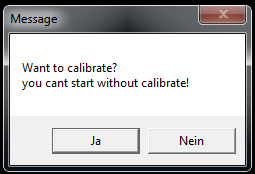
\includegraphics[width=\textwidth/3]{bilder/Calibrate-Popup.png}
\end{figure}\\
Mit dem Drücken des 'Ja'-Knopfes wird ein Signal Richtung der Kamerakalibrierung geschickt und diese wird gestartet. Sollte 'Nein' gedrückt worden sein, so wird das Programm geschlossen.
Nach der Kalibrierung wird ein weiteres Pop-up Fenster angezeigt, ob man das Spiel nun starten möchte. Wenn 'Ja' gedrückt wird, dann wird das ganze Spielfeld angezeigt. 
 \begin{figure}[h]
	\centering
	\caption{StartGame-Pop-up}
	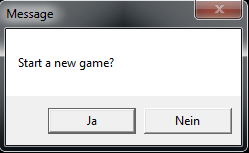
\includegraphics[width=\textwidth/3]{bilder/startGame-Popup.png}
\end{figure}\\
Nebenbei werden auch die Labels für den CurrentPlayer sowie des Balltypen angezeigt.
Das Spiel kann nun mit einem Queue gestartet werden. Hierbei muss man mit dem Queue versuchen die weiße Kugel anzustoßen. Wichtig dabei ist, dass die Kamera eingeschaltet bleiben muss.
\\\\\\
Als zusätzliche Funktion, hat der Spieler die Möglichkeit mit der Maus zu spielen, indem er diese entsprechend gegen die weißen Kugel schlägt.
\begin{figure}[h]
	\centering
	\caption{Maus Funktion}
	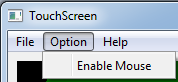
\includegraphics[width=\textwidth/3]{bilder/option-MenuBar.png}
\end{figure}\\\\
Unter dem Menüpunkt 'File' hat der Benutzer die Möglichkeit das Spiel zurück zu setzen bzw. ein neues Spiel zu starten.
\begin{figure}[h]
	\centering
	\caption{Start New Game}
	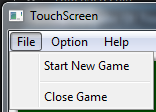
\includegraphics[width=\textwidth/3]{bilder/File-MenuBar.png}
\end{figure}\\

\subsection{Zusammenfassung}
In der allgemeinen Übersicht wurde in diesem Kapitel die Benutzerinteraktion vereinfacht, um dem Nutzer eine möglichst simple Steuerung mit der Anwendung zu gewährleisten. Dies wurde mit Hilfe von Popups und Interaktionsmöglichkeiten über Buttons in der Menubar ermöglicht.